%\documentclass[12pt,xcolor=dvipsnames,mathserif]{beamer}
\documentclass[12pt,xcolor=dvipsnames,handout,mathserif,aspectratio=169]{beamer}

\usepackage{hyperref}

\usepackage{pgfpages}
\usepackage{colortbl}
\usepackage{multirow}
\usepackage{eurosym}

%\pgfpagesuselayout{2 on 1}[border shrink=2.5mm]
%\pgfpageslogicalpageoptions{1}{border code=\pgfusepath{stroke}}
%\pgfpageslogicalpageoptions{2}{border code=\pgfusepath{stroke}}


% Specify theme
%\usetheme{Madrid}
\usetheme{Boadilla}
% See deic.uab.es/~iblanes/beamer_gallery/index_by_theme.html for other themes

% Specify base color
%\usecolortheme[named=OliveGreen]{structure}
\usecolortheme[named=RoyalBlue]{structure}
% See http://goo.gl/p0Phn for other colors

% Specify other colors and options as required
\setbeamercolor{alerted text}{fg=Red}
\setbeamertemplate{items}[square]

% Specify some useful short commands
\newcommand{\bbl}[1]{{\color{NavyBlue} \textbf{#1}}}
\newcommand{\bre}[1]{{\color{red} \textbf{#1}}}
\newcommand{\bgr}[1]{{\color{PineGreen} \textbf{#1}}}
\newcommand{\un}{\texttt{\char`_}}
\newcommand{\tcb}{\textcolor{blue}}
\newcommand{\EE}{\mathrm{I\!E\!}}
\newcommand{\PP}{\mathbb{P}}


\newcommand{\tc}{\textcolor}
\newcommand{\tcbl}{\textcolor{bluelight}}


% Title and author information
\title[Introductory Statistics with Excel]{Introductory Statistics with Excel}
\author[Andrew Parnell]{Andrew Parnell}
\institute[UCD]{University College Dublin \begin{center} 
\includegraphics[width=1.5cm]{UCDlogo.pdf}\end{center} }
\date[Class 6]{Class 6 - Linear regression and control charts}
%\date{Lecture 2 -- part 1}

\begin{document}

\titlepage

\begin{frame}{Learning outcomes}

In this class we will cover
\begin{itemize}
\item Correlation and bivariate data
\item Linear regression models
\item Simple control charts
\end{itemize}

\end{frame}

\begin{frame}{Relationships between variables}

It is very rare for variables to change in \bre{isolation}. Most often, multiple variables change \bbl{simultaneously}, and we are interested in understanding their \bgr{relationship} and possibly \bbl{predicting} one or more variables from the others.\\
\vspace{0.5cm}
\pause
In this class we will learn some methods for \bgr{quantifying} the relationships between quantitative and qualitative variables.\\
\vspace{0.5cm}
\pause
We have already met some graphical methods for performing some of these tasks, including \bbl{scatter plots}, \bre{box plots} and \bgr{histograms}.

\end{frame}

\begin{frame}{Relationships between quantitative variables}

Example: some data measure the age of 30 drivers together with the maximum distance at which they could read a signpost. A scatter plot of the data is shown below
\begin{center}
\includegraphics[width=0.4\textwidth]{agedist.pdf}
\end{center}
\pause
This is an example of a \bbl{negative statistical relationship}; in general as age goes up the maximum readability distance goes down
\end{frame}

\begin{frame}{Looking for patterns in scatter plots}
Some questions to ask:
\begin{itemize}
\item What is the \bbl{average pattern}? Is it a linear relationship (a straight line) or is it curved?
\item What is the direction of the pattern? Is it a \bgr{positive} or \bre{negative} relationship?
\item How much do the individual points \bre{vary} from the average pattern?
\item Are there any \bre{unusual} data points (outliers)?
\end{itemize}
\end{frame}

\begin{frame}{Linear and non-linear relationships}

Not all relationships between quantitative variables are linear. Consider the following examples:
\begin{itemize}
\item The relationship between height and age
\item The relationship between car age and selling price
\end{itemize}
\pause
\vspace{0.2cm}
There are two analyses we often perform with pairs of quantitative variables. The first is to calculate the strength of the linear relationship between the two variables, known as the \bbl{correlation}. The second is to try and predict one of the variables from the other, known as \bbl{linear regression}

\end{frame}

\begin{frame}[fragile]{}
\bbl{\Huge Correlation}\\ 
\vspace{0.5cm}
\end{frame}


\begin{frame}{Calculating the correlation coefficient}

The Pearson \bbl{correlation coefficient} (often written as $r$) measures the strength and direction of a \bre{linear} relationship by a number between 1 and -1. 
\begin{itemize}
\item A number close to $r=1$ or $r=-1$ indicates that the relationship (as seen in a scatter plot) is almost perfectly linear
\pause
\item A number close to $r=0$ indicates that there is no linear relationship between the two variables
\pause
\item If the value is positive ($r>0$) the two variables tend to increase together. If it is negative ($r<0$) then as one variable increases the other decreases
\end{itemize}

\end{frame}

\begin{frame}{Calculating the correlation coefficient}

If we label one variable as $x$ and the other as $y$ so that the observations are in pairs $(x_{1},y_{1}),\; (x_{2},y_{2}),\ldots, (x_{n},y_{n})$, the correlation coefficient can be calculated as:
$$r = \frac{1}{n-1} \sum_{i=1}^{n} \left( \frac{x_{i}-\bar{x}}{s_{x}} \right) \left( \frac{y_{i}-\bar{y}}{s_{y}} \right)$$
where $\bar{x}$ and $\bar{y}$ are the means of the $x$ and $y$ variables, and $s_x$ and $s_{y}$ are the standard deviations of the $x$ and $y$ variables respectively.\\
\pause
\vspace{0.2cm}
Note that the terms inside the brackets are the \bgr{standardised data points} which we met in lecture 3 when we met the normal distribution

\end{frame}

\begin{frame}{Some examples}

The age/distance data set we met at the start of this lecture has a correlation value of $r=-0.795$
\begin{center}
\includegraphics[width=0.5\textwidth]{agedist.pdf}
\end{center}
%Let's take a look at some of the data collected earlier in the course
\end{frame}

\begin{frame}{Some important notes about correlation}

\begin{itemize}
\item If you look at the formula for calculating the correlation coefficient you can see how a positive or negative value of $r$ can be obtained. For example, if the standardised $x$-value is above the $x$ mean and standardised $y$-value is above the $y$ mean then you are multiplying two positive values together. Similarly, if they are both below their respective means you are multiple negative values together
\pause
\item Note that just because two variables are correlated, it does not mean that one is caused by the other. There may be a \bre{confounding} variable
\pause
\item There are different ways to calculate the $r$ value, and different versions of it for qualitative or ordinal variables
\end{itemize}

\end{frame}

\date{Lecture 6 -- Part 3}

\begin{frame}[fragile]{}
\bbl{\Huge Linear regression}\\ 
\vspace{0.5cm}
\end{frame}


\begin{frame}{Linear regression}

Suppose now we want to predict one variable from another. As in Class 2, we call the variable we want to predict the \bbl{response variable} and the remaining variable the \bgr{explanatory variable}. This is a common problem in science:
\begin{itemize}
\item We might want to predict whether someone has a disease based on the results of a medical test that they take
\item We might want to predict how big a product's sales will be based on the amount spent on advertising it
\end{itemize}
\pause
If we are happy to assume a linear relationship we create a \bgr{statistical model}:
$$\mbox{response} = a + b \times \mbox{explanatory} + \mbox{residual} $$
where $a$ is the \bbl{intercept} and $b$ is the \bgr{slope}, both to be estimated from the data
\end{frame}

\begin{frame}{Fitting the regression equation}

One way of estimating the values of the slope and intercept is via \bgr{least squares} where we try to minimise the squared differences between the estimated values from the model (i.e. ignoring the residual component) and the true values of $y$. 
\begin{center}
\includegraphics[width=0.6\textwidth]{agedistreg.pdf}
\end{center}
\end{frame}

\begin{frame}{Some notes about linear regression}

\begin{itemize}
\item The vertical distances between the data points and the fitted line are called \bre{residuals} as they represent the leftover variation in the data points beyond that of the fitted linear regression model
\pause
\item Often the square of the correlation coefficient ($r^2$) is reported along with the slope and the intercept. This is often used to illustrate the \bbl{proportion of variation `explained' by the linear regression}. 
\pause
\item We should be very careful about \bre{extrapolating} our line beyond the $x$ range of the data. 
\pause
\item The name \bgr{regression} comes from Francis Galton who used it to derive the relationships between the heights of parents and children. He originally called the method `reversion'
\end{itemize}
\end{frame}

%\begin{frame}{Graph of the week}
%\begin{center}
%\includegraphics[width=\textwidth]{PredictedVote.pdf}
%\end{center}
%\end{frame}

\begin{frame}{Measuring relationships between categorical variables}

We have already met methods for presenting categorical variables with two categories, such as \bgr{cross-tabulations} and \bbl{bar charts}.\\
\vspace{0.2cm}
Example: deaths on the Titanic
\begin{center}
\begin{tabular}{l|cccc}
\hline
Class & 1st & 2nd & 3rd & Crew \\
\hline
Survived & 203 & 118 & 178 & 212 \\
Died & 122 & 167 & 528 & 673 \\
\hline
Total & 325 & 285 & 706 & 885 \\
\hline
\end{tabular}
\end{center}
What can we say about the relationship between the class of passenger and the survival rate?
\end{frame}

\begin{frame}{Risk and relative risk}

The first thing we can compute is the \bgr{risk} (or \bgr{baseline risk}) of being in an undesirable category:
$$\mbox{Risk} = \frac{ \mbox{Number in category} }{ \mbox{Total number in group} }$$
For example, the risk of a 1st class passenger dying is $\frac{122}{325} \approx 0.375$
\pause
\vspace{0.2cm}
Next, we could calculate the \bgr{relative risk} which is the ratio of risks in two different groups:
$$\mbox{Relative Risk} = \frac{ \mbox{Risk in category 1} }{ \mbox{Risk in category 2} }$$
For example, the relative risk of a 3rd class passenger compared to a first class passenger is $\frac{0.748}{0.375} \approx 2$. Thus you were approximately \bre{twice as likely to die} if you were in 3rd class compared to 1st!

\end{frame}

\begin{frame}{Odds and Odds ratios}

The \bbl{odds} of an event compare the chance that it does not happen with the chance that it does. We are used to seeing odds written as `$a$ to $b$', for example in horse racing you might see a horse given as 3 to 1 to win the race. \\
\vspace{0.2cm}
\pause
We can transform odds into probabilities by calculating $\frac{b}{a+b}$ in the odds. Thus a 3 to 1 horse has probability 0.25 of winning the race. 
Some notes:
\begin{itemize}
\item Bookmakers usually publish the odds \bbl{against} an event rather than the events \bgr{for} an event. This can make things quite confusing
\pause
\item The odds given by bookmakers, when transformed into probabilities, don't usually add to 1. The difference is their profit margin!
\end{itemize}
\vspace{0.2cm}
The \bgr{odds ratio} is calculated by dividing the odds in two different categories.

\end{frame}

\begin{frame}{A summary slide on risk and odds}

\begin{block}{}
Suppose you have the following table:
\begin{center}
\begin{tabular}{lccc}
\hline
 & \multicolumn{2}{c}{Response Variable} & \\
Explanatory variable & Response 1 & Response 2 & Total \\
\hline
Category of interest & $A_1$ & $A_2$ & $T_A$ \\
Baseline category & $B_1$ & $B_2$ & $T_B$ \\
\hline
\end{tabular}
\end{center}
Now:
\begin{itemize}
\item The \bgr{risk} (of response 1) for the category of interest is $A_1/T_A$
\item The \bgr{odds} (of response 1 to response 2) is $A_1$ to $A_2$
\item The \bbl{relative risk} is $\frac{A_1/T_A}{B_1/T_B}$
\item The \bbl{odds ratio} is $\frac{A_1/A_2}{B_1/B_2}$
\end{itemize}

\end{block}
\end{frame}

\begin{frame}{Common mistakes with risk}

\begin{block}{}
A recent study of 6000 women claims that drinking 5 cups of coffee per day reduces women's risk of breast cancer by 57\%\footnote{\url{http://www.dailymail.co.uk/health/article-1385763/Five-cups-coffee-day-protect-breast-cancer.html}}.
\end{block}
Should you start drinking a bucket of coffee a day?\\
\pause
\vspace{0.2cm}
\begin{itemize}
\item We should always get the sample size and the \bgr{baseline risk}. It might be that such a small proportion of people suffer from breast cancer that a 57\% change doesn't make much difference
\item Remember all the other ways that statistical studies can fool us: confounding variables, study limitations, etc
\item Revisit lecture 1: disaster in the skies
\end{itemize}
\end{frame}

\begin{frame}[fragile]{}
\bbl{\Huge Control charts}\\ 
\vspace{0.5cm}
\end{frame}


\frame{
\frametitle{Quality Control}
\begin{itemize}
 \item Variability is inevitable in any manufacturing process.\\
 e.g. Two screws made by the same machine and from the same raw materials will show some variation in length and diameter.
 
 \item As in the previous statistical models we have met, variability may be partitioned into \bbl {residual variation} and \bbl{assignable cause}.
 
\item Residual variation is that which is left over, i.e. beyond simple explanation.

\item Assignable causes could be worn machine parts, poorly trained operators or the production environment. 

\pause

\item If the variability in a production process is only due to residual variation then the process is said to be \bbl{in control}.
\end{itemize}

}

\frame{
\frametitle{Control Charts}
\begin{itemize}
 \item Control charts consist of a \bbl{central line} and upper and lower \bbl{control limits}.
 
 \item The observed values are plotted and if any fall outside the control limits, the process is said to be \bbl{out of control}.
 \pause
 
 \item Control limits and the central line can be estimated from data collected when the process is known to be in control.
\end{itemize}
\pause
\begin{block}{Important}
 Control limits are appropriate only for analysing past data (data used in their calculation). They can be used for future data only when the process is in control and/or when the limits have been modified.
\end{block}
}


\frame{
\frametitle{Example}
\begin{center}
 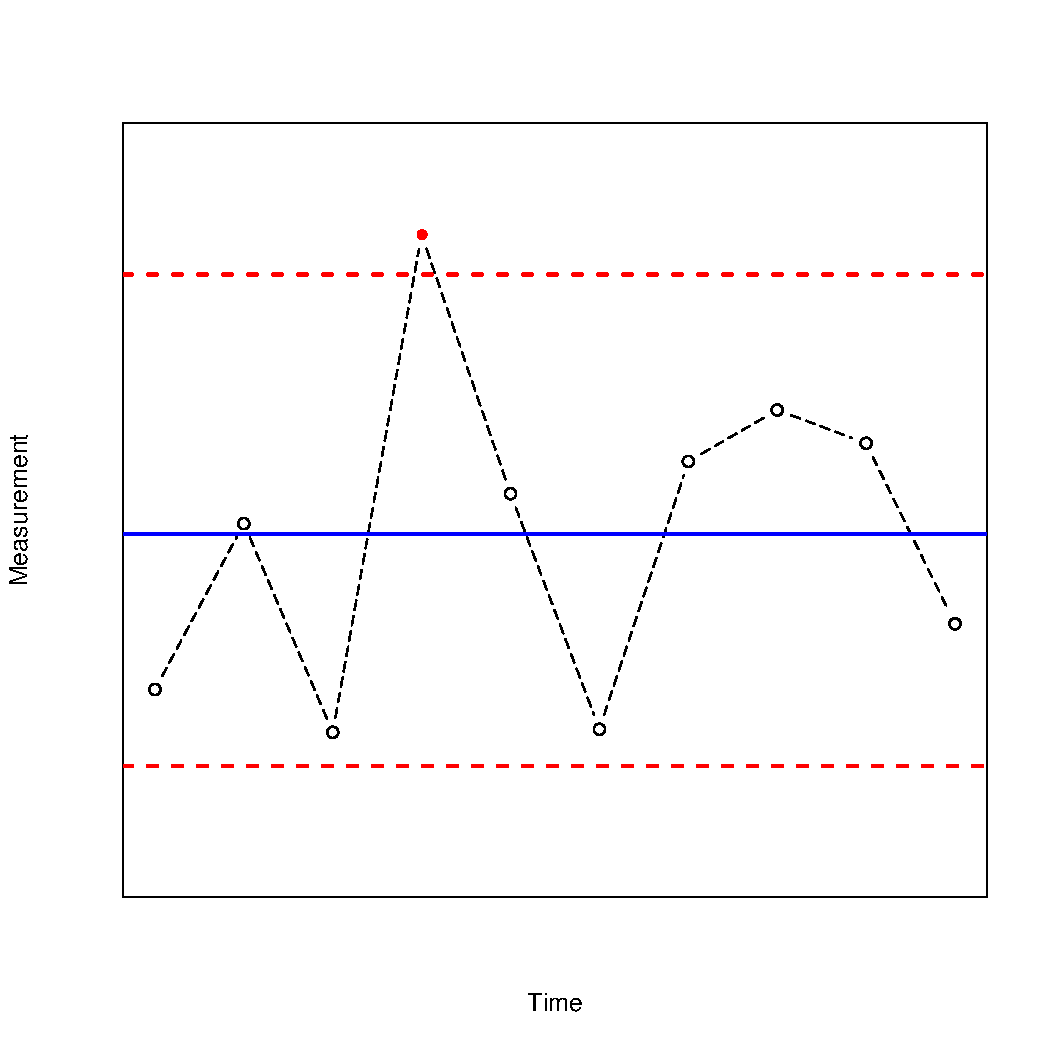
\includegraphics[width=0.5\textwidth]{BasicControlChart.pdf}
\end{center}
}

\frame{
\frametitle{Chart Setup}
\begin{itemize}
 \item When control charts are first applied the process may not be in control.
 \item Even if it is in control, the behaviour of the process will not yet be fully understood. \item Data needs to be collected from the process and any assignable causes of variation removed. This is the \bbl{chart setup} stage.
 \item After the process has been operating in control for some time, a large amount of data is available and control charts may be used to monitor the process.
 \item We will focus on the process monitoring stage here.
\end{itemize}
}

\frame{
\frametitle{Benefits of Control Charts}
\vspace{-0.25cm}
\begin{itemize}
 \item \bbl{Improve productivity:} Scrap and rework are reduced by monitoring a process with control charts.
 
 \pause
 
 \item \bbl{Defect prevention:} An in control process, producing goods consistently correctly, reduces the amount of defective produce.
 
 \pause
 
 \item \bbl{Prevent unnecessary process adjustments:} If processes are only checked periodically, operators often overreact to random error. This is not the case if the process is monitored continuously.
 
 \pause
 
 \item \bbl{Diagnostic information:} An experienced engineer can often use a control chart (in tandem with other information) to diagnose a process problem.
 
 \pause
 
 \item \bbl{Process capability:} A control chart monitors important process parameters and their stability over time. This information can be used to assess if the process is fit for purpose or not.
\end{itemize}

}

\frame{
\frametitle{Control Chart for Means: $\bar{x}$-chart}
\begin{itemize}
 \item Rather than one measurement at each time point, take a number of measurements, $n$, at each time point and calculate their sample mean $\bar{x}$.
 \pause
 
 \item By the central limit theorem the sample mean should vary about the true process mean $\mu$ with standard deviation $\sigma$, and should fall within the interval $\mu \pm 3\frac{\sigma}{\sqrt{n}}$ with a very high probability ($> 0.99$) like a wide confidence interval
 \pause
 
 \item The limits of this interval will be the upper control limit (UCL) and lower control limit (LCL).

\end{itemize}
}

\frame{
\frametitle{Control Chart for Means: $\bar{x}$-chart}
\begin{itemize}
\item As we almost never know the true value of $\mu$ or $\sigma$ these must be estimated from some collected data. 

 \item Let the time points be denoted by $i=1, \ldots, k$. Recall that $n$ measurements are taken at each time point.
 \pause
 
 \item The mean at each time point is denoted by $\bar{x}_i = \sum_j x_{ij}/n$. 
 \pause
 
 \item The center line is estimated by the grand mean:
 $$\bar{\bar{x}} = \frac{\sum_{i=1}^k \bar{x}_i}{k}$$
\end{itemize}
}

\frame{
\frametitle{Control Chart for Means: $\bar{x}$-chart}
\begin{itemize}
 \item It is standard in control charts to use $R_i$, the range at each time point $i$, to estimate $\sigma$.
 $$\hat{\sigma} = \frac{\bar{R}}{d_2} = \frac{\sum_{i=1}^{k}R_i/k}{d_2}$$
 where $d_2$ is a constant depending on $n$. (Values of $d_2$ for differing $n$ are at the back of these slides)
 \pause
 
 \item Thus:
 $$3\frac{\sigma}{\sqrt{n}} \approx 3\frac{\hat{\sigma}}{\sqrt{n}} = \frac{3(\bar{R}/d_2)}{\sqrt{n}} = \frac{3}{d_2\sqrt{n}}\bar{R} = A_2\bar{R}$$
 where $A_2 = \frac{3}{d_2\sqrt{n}}$
 \end{itemize}
}

\frame{
\frametitle{Control Chart for Means: $\bar{x}$-chart}
\begin{block}{Summary}
\begin{itemize}
 \item Center line : $\bar{\bar{x}} = \frac{\sum_{i=1}^k \bar{x}_i}{k}$
 \item UCL: $\bar{\bar{x}} + A_2 \bar{R}$
 \item LCL: $\bar{\bar{x}} - A_2 \bar{R}$
\end{itemize}
where
\begin{itemize}
 \item $k = $ number of samples, each of size $n$.
 \item $\bar{x}_i = $ mean of $i^{th}$ sample.
 \item $R_i = $ range of $i^{th}$ sample.
 \item $\bar{R} = \sum_{i=1}^{k}R_i/k$ 
 \end{itemize} 
\end{block}
}

\frame{
\frametitle{Interpretation}
\begin{description}
 \item[Out of control:] One or more of the sample points fall outside the control limits. This indicates there may be some problem with the production process and should be investigated. \bbl{Trends} in the process mean may also indicate the presence of some assignable variation.
 
 \pause
 \item[In control:] All sample points fall within the control limits. There may still be problems with the process but it is most likely better to leave the process alone than to look for problems that may not exist.
\end{description}
}

\frame{
\frametitle{Example:}
The following are the sample means and ranges of 20 samples, each consisting of the weight of 5 castings in ounces. Construct an $\bar{x}$-chart from these data.
\begin{center}
 \begin{tabular}{rrrr}
  \hline
$\bar{x}$ & $R$ & $\bar{x}$ & $R$ \\ 
  \hline
4.24 & 0.09 & 4.20 & 0.21 \\ 
  4.18 & 0.12 & 4.25 & 0.20 \\ 
  4.26 & 0.14 & 4.25 & 0.17 \\ 
  4.21 & 0.24 & 4.21 & 0.07 \\ 
  4.22 & 0.15 & 4.19 & 0.16 \\ 
  4.18 & 0.28 & 4.23 & 0.16 \\ 
  4.23 & 0.06 & 4.27 & 0.19 \\ 
  4.19 & 0.15 & 4.22 & 0.20 \\ 
  4.21 & 0.09 & 4.20 & 0.12 \\ 
  4.18 & 0.15 & 4.19 & 0.16 \\ 
   \hline
\end{tabular}
\end{center}


}

\frame{
\frametitle{Example}
\begin{itemize}
 \item Center line: $\bar{\bar{x}} = 4.216$
 \item UCL: $\bar{\bar{x}} + A_2\bar{R} = 4.216 + (0.58)(0.156) = 4.306$
 \item LCL: $\bar{\bar{x}} - A_2\bar{R} = 4.216 - (0.58)(0.156) = 4.125$
\end{itemize}
\pause
\begin{center}
 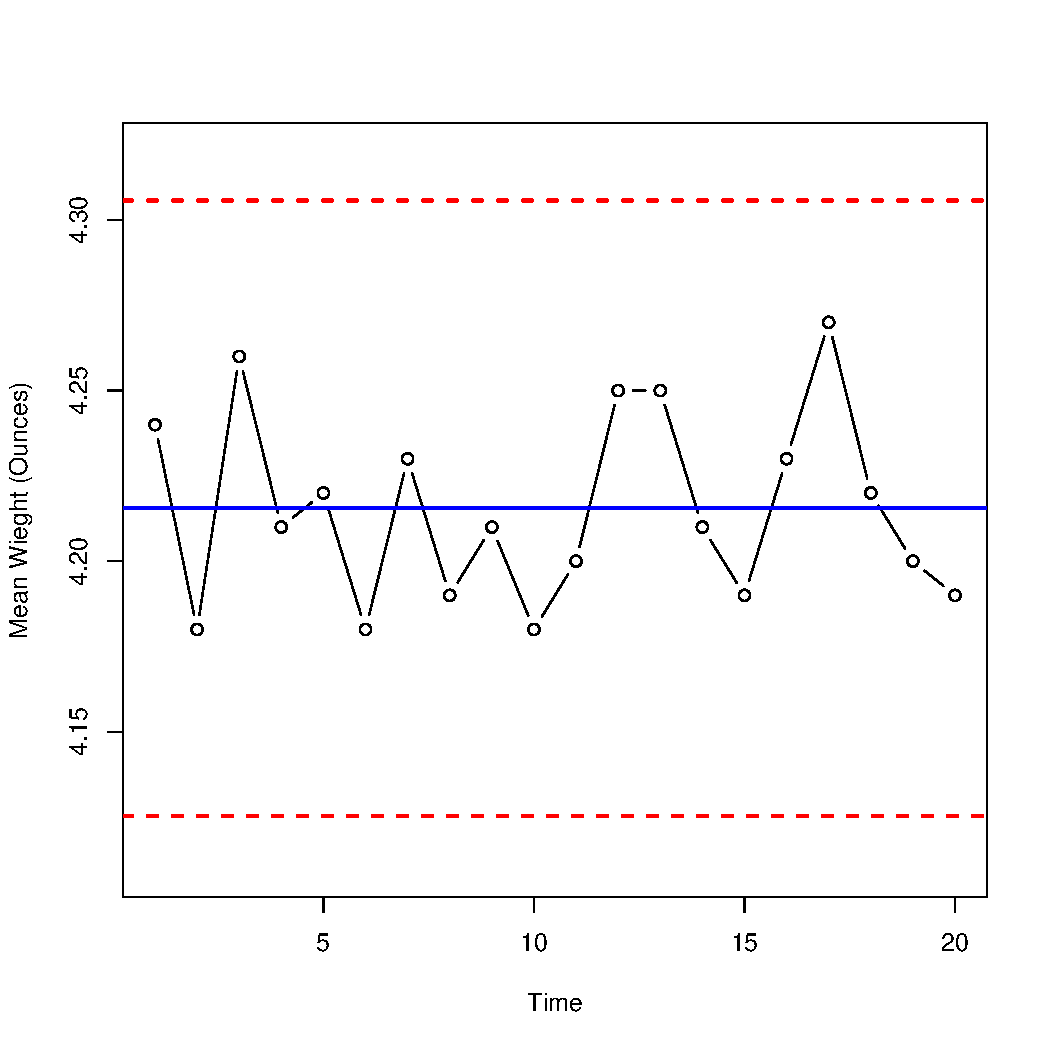
\includegraphics[width=0.4\textwidth]{ex1_xbarChart.pdf}
\end{center}
}

\frame{
\frametitle{Control Chart for Process Variation: $R$-Chart}
\begin{itemize}
 \item Quality control engineers also need to monitor the variability of a process. 
  
 \item Large variability in a process will produce non-uniform, inferior products.
  
 \pause
 \item Changes in the variability of a process can also be indicative of assignable variation.
  
 \pause
 \item The variability of a process can be monitored using an $R$-chart.
\end{itemize}
}

\frame{
\frametitle{Control Chart for Process Variation: $R$-Chart}
\begin{block}{Summary}
\begin{itemize}
 \item Center line : $\bar{R}$
 \item UCL: $D_4\bar{R}$
 \item LCL: $D_3\bar{R}$
\end{itemize}
where $D_3$ and $D_4$ are constant related to $n$, the size of the individual samples. \\(Values of $D_3$ and $D_4$ for differing $n$ are at the back of these slides)
\end{block}
}

\frame{
\frametitle{Control Chart for Process Variation: $R$-Chart}
\begin{itemize}
 \item $R$-charts can be interpreted in the same way as $\bar{x}$ charts. If any points fall outside the control limits the process is said to be out of control. 
 \pause
 
 \item Trends in the variability of a process may also indicate the presence of some assignable variation.
 \begin{itemize}
  \item Increasing/decreasing variability.
  \item Large numbers of consecutive points above/below the center line.
 \end{itemize}

 \pause
 
 \item Only if the variability is in control ($R$-chart) should the quality measurement ($\bar{x}$-chart) be checked. Variabilty which is out of control may mask problems with the quality measurement.
\end{itemize}
}

\frame{
\frametitle{Example}
\begin{itemize}
 \item Center line: $\bar{R} = 0.156$
 \item UCL: $D_4 \bar{R} = (2.11)(0.156) = 0.328$
 \item LCL: $D_3 \bar{R} = (0)(0.156) = 0$
\end{itemize}
\begin{center}
 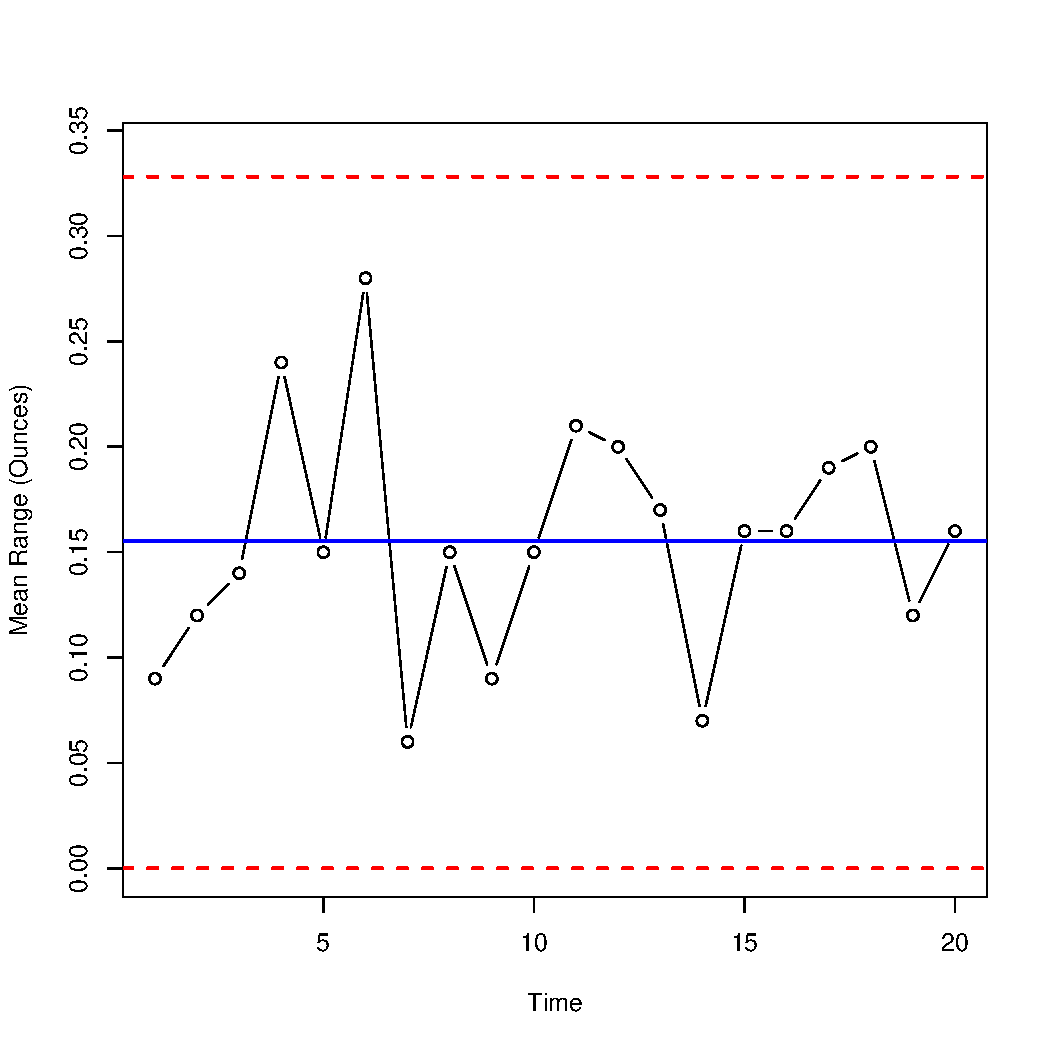
\includegraphics[width=0.4\textwidth]{ex1_RChart.pdf}
\end{center}
}

\begin{frame}{Summary of class 6}

\begin{itemize}
\item Correlation and linear regression very useful for quantifying the \bbl{relationship} between two \bgr{quantitative} variables
\item Relative and absolute risk/odds useful for quantifying \bbl{categorical} relationships
\item $\bar{x}$-bar control charts useful for quantifying \bre{mean} problems, and $R$-charts useful for quantifying \bre{variability} problems
\end{itemize}
\end{frame}

\begin{frame}{Summary of course}

\begin{itemize}
\item You now have had reasonable exposure to a good chunk of 20th century statistical methodology
\item If you want to update yourself for the 21st century you need to:
\begin{enumerate}
\item Learn R or Python
\item Learn about Bayesian statistics (and hierarchical modelling)
\item Take a course in machine learning 
\end{enumerate}
\end{itemize}
\end{frame}

\frame{
\frametitle{Control Chart Constants}
\begin{table}
\tiny
 \centering
\begin{tabular}{rrrrrrrr}
  \hline
n & A2 & A3 & d2 & D3 & D4 & B3 & B4 \\ 
  \hline
  2 & 1.88 & 2.66 & 1.13 & 0.00 & 3.27 & 0.00 & 3.27 \\ 
    3 & 1.02 & 1.95 & 1.69 & 0.00 & 2.57 & 0.00 & 2.57 \\ 
    4 & 0.73 & 1.63 & 2.06 & 0.00 & 2.28 & 0.00 & 2.27 \\ 
    5 & 0.58 & 1.43 & 2.33 & 0.00 & 2.11 & 0.00 & 2.09 \\ 
    6 & 0.48 & 1.29 & 2.53 & 0.00 & 2.00 & 0.03 & 1.97 \\ 
    7 & 0.42 & 1.18 & 2.70 & 0.08 & 1.92 & 0.12 & 1.88 \\ 
    8 & 0.37 & 1.10 & 2.85 & 0.14 & 1.86 & 0.18 & 1.81 \\ 
    9 & 0.34 & 1.03 & 2.97 & 0.18 & 1.82 & 0.24 & 1.76 \\ 
   10 & 0.31 & 0.97 & 3.08 & 0.22 & 1.78 & 0.28 & 1.72 \\ 
   11 & 0.28 & 0.93 & 3.17 & 0.26 & 1.74 & 0.32 & 1.68 \\ 
   12 & 0.27 & 0.89 & 3.26 & 0.28 & 1.72 & 0.35 & 1.65 \\ 
   13 & 0.25 & 0.85 & 3.34 & 0.31 & 1.69 & 0.38 & 1.62 \\ 
   14 & 0.23 & 0.82 & 3.41 & 0.33 & 1.67 & 0.41 & 1.59 \\ 
   15 & 0.22 & 0.79 & 3.47 & 0.35 & 1.65 & 0.43 & 1.57 \\ 
   16 & 0.21 & 0.76 & 3.53 & 0.36 & 1.64 & 0.45 & 1.55 \\ 
   17 & 0.20 & 0.74 & 3.59 & 0.38 & 1.62 & 0.47 & 1.53 \\ 
   18 & 0.19 & 0.72 & 3.64 & 0.39 & 1.61 & 0.48 & 1.52 \\ 
   19 & 0.19 & 0.70 & 3.69 & 0.40 & 1.60 & 0.50 & 1.50 \\ 
   20 & 0.18 & 0.68 & 3.73 & 0.41 & 1.58 & 0.51 & 1.49 \\ 
   21 & 0.17 & 0.66 & 3.78 & 0.42 & 1.57 & 0.52 & 1.48 \\ 
   22 & 0.17 & 0.65 & 3.82 & 0.43 & 1.57 & 0.53 & 1.47 \\ 
   23 & 0.16 & 0.63 & 3.86 & 0.44 & 1.56 & 0.55 & 1.46 \\ 
   24 & 0.16 & 0.62 & 3.90 & 0.45 & 1.55 & 0.56 & 1.45 \\ 
   25 & 0.15 & 0.61 & 3.93 & 0.46 & 1.54 & 0.56 & 1.44 \\ 
   \hline
\end{tabular}
\end{table}
}




\end{document}
